% siminos/CLE/movingFrames.tex


\subsection{Moving frames}
\label{sec:mf}

In this section we present the method of moving frames of
Cartan\rf{CartanMF} in the formulation of Fels and
Olver\rf{FelsOlver98,FelsOlver99}, also \cf~\refref{OlverInv}
for a pedagogical exposition and the proofs of theorems
listed here. Its purpose is to generate functionally
independent invariants for the action of a group $\Group$ on
a manifold $\Manif$ under certain assumptions. Here we will
describe how, and to what extend, the invariants generated can be utilized in 
symmetry reduction problems.

In the following let $\Group$ be $r$-dimensional and act on a
$n$-dimensional manifold $\Manif$.
A moving frame is a smooth $\Group$-equivariant mapping
$\rho$ from $\Manif$ to the $\Group$, that is to the group
parameters.
\ES{perharps not needed: One distinguishes between left moving frames for which the
equivariance condition is $\rho(\gamma x)=\gamma\rho(x)\,,\
x\in\Manif\,,\ \gamma\in\Group$ and right moving frames for
which the equivariance condition is $\rho(\gamma
x)=\rho(x)\gamma^{-1}\,,\ x\in\Manif\,,\ \gamma\in\Group$.
}

As shown in \refref{FelsOlver98} a moving frame exists 
in a neighborhood of a point $x\in\Manif$ if and only if 
$\Group$ acts freely and regularly  near x. For the practical
construction of a moving frame for an $r-$dimensional Lie group
$\Group$ we will need to introduce the
notion of a \emph{slice}, an $(n-r)$-dimensional submanifold $K$
of $\Manif$ such that $K$ intersects each group orbit
transversally and at most once. Here we prefer the term slice 
to \emph{cross-section} used by Fels and Olver\rf{FelsOlver98} 
as the latter has a well established usage in the physics 
literature. Moreover, we wish to emphasize the local nature
of the slices constructed here. As the existense of a slice
depends on the regularity of the group action\rf{FelsOlver98}
and thus for most interesting group actions a slice is bound to
exist only locally.

\begin{proposition}%[\rf{OlverInv}]
 \label{pro:crossExists}
 If a Lie group $\Group$ acts regularly on a manifold 
 $\Manif$, then one can construct a
 local {\csection} passing through any point $x\in \Manif$.
\end{proposition}\ES{Is it if and only if?}
For proof see \refref{FelsOlver98}

The definition of a slice provides a means of constructing a moving frame.
In particular, let $K\subset\Manif$ be a {\csection}. For $x\in \Manif$, let
$\gamma=\rho(x)$ be the unique group element that maps $x$
to the {\csection}: $g x = \rho(x) x\, \in K$. Then
$\rho:\Manif\rightarrow \Group$ is a right moving frame\rf{FelsOlver98}.

A {\csection} $K$ can be defined by means of level sets of
functions $K_i(x)=c_i$, where $x\in V$ and $i=1,\ldots,r$. If
the $K_i(x)$ coincide with the local coordinates $x_i$ on the
manifold $V$, \ie~$K_i(x)=x_i$, then we call $K$ a
\emph{coordinate \csection}.

\begin{example}
Consider the standard action of $\SOn{2}$ on \Rls{2}:
\beq
	(x,y) \mapsto (x\cos\theta -y \sin\theta,\,x\sin\theta +y \cos\theta )
\eeq
which is regular on $\Rls{2}\backslash\{0\}$. Thus we can define
a {\csection} by, for instance, the
positive $y$ axis: $x=0,\,y>0$.
We can now construct a moving frame as follows. We write out
explicitly the group transformations:
\begin{subequations}
\begin{align}
 	\overline{x} &= x \cos\theta - y \sin\theta\label{eq:explSO2stnd1}\cont
	\overline{y} &= x \sin\theta + y \cos\theta\label{eq:explSO2stnd2}\,.
\end{align}
\end{subequations}
Then set $\overline{x}=0$ and solve \refeq{eq:explSO2stnd1} for the group
parameter to obtain the moving frame
\beq
	\theta=\tan^{-1}\frac{x}{y}
	\label{eq:SO2stndMF}
\eeq
which brings any point  back to the {\csection}.
\footnote{Implementation note: Here it is important that
$\tan^{-1}$ distinguishes quadrants on the $(x,y)$ plane so
that we get the correct geometric operation.}
Substituting \refeq{eq:SO2stndMF} in the remaining equation,
we get the $\SOn{2}$-invariant expression
\beq
	\overline{y} = \sqrt{x^2+y^2}\,.
\eeq
\end{example}

The above \emph{normalization} procedure for the computation of
invariants can be applied in much more general situations as follows. 
\ES{Already implicit, drop: Assume $\Group$ acts (locally) freely
    \ES{The condition of free action can be
    relaxed\rf{OlverInv}.}
on \Manif\  and thus $\Group$-orbits have the same dimension,
say $r$, as $\Group$.
}  
Choose a coordinate {\csection} $K=\{x_1=c_1,\ldots,x_r=c_r\}$ defined by the first $r$
coordinates (relabel coordinates as necessary). 
\ES{irrelevant in practice:
Introduce
local coordinates $g=(g_1,\ldots,g_r)$ on $\Group$ in the
neighborhood of the identity.} 
Write the group transformations as
\beq
	\overline{x}= g \cdot x = w(g,x)\,.
	\label{eq:transNorm}
\eeq
Equating the first $r$ components of the function $w$ to the
constants in the definition of the {\csection} $K_i(x)=c_i$
yields the \emph{normalization equations} for $K$:
\beq
	\overline{x}_1=w_1(g,x)=c_1,\ldots,\overline{x}_r=w_r(g,x)=c_r\,.
	\label{eq:normalization}
\eeq
The normalization equations \refeq{eq:normalization}
can always be solved\rf{FelsOlver98} for the group parameters in terms of
$x$, yielding the moving frame associated with $K$:
$g=\gamma(x)$. Substitution of the moving frame equation back
in \refeq{eq:transNorm} will yield the $n-r$
\emph{fundamental invariants}, that is functionally independent
invariants that can be used as a basis in which any other invariant
can be expressed. Thus the fundamental invariants serve to distinguish
group orbits in the neighborhood of the {\csection}, \ie~two points
lie on the same group orbit if and only if all the
fundamental invariants agree. For proof
\cf~\refrefs{FelsOlver98,FelsOlver99}.

\subsubsection{Moving frame for \CLe}
\label{sec:CLeMF}


%%%%%%%%%%%%%%%%%%%%%%%%%%%%%%%%%%%%%%%%%%%%%%%%%%%%%%%%%%%%%%%%
\begin{figure}[ht]
\begin{center}
  (\textit{a})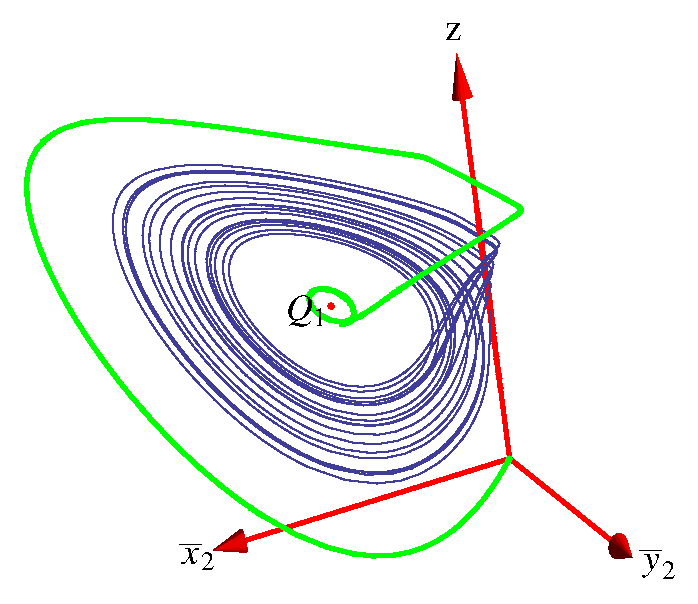
\includegraphics[width=0.35\textwidth]{../figs/CLEmfXYZ}
~~~~(\textit{b})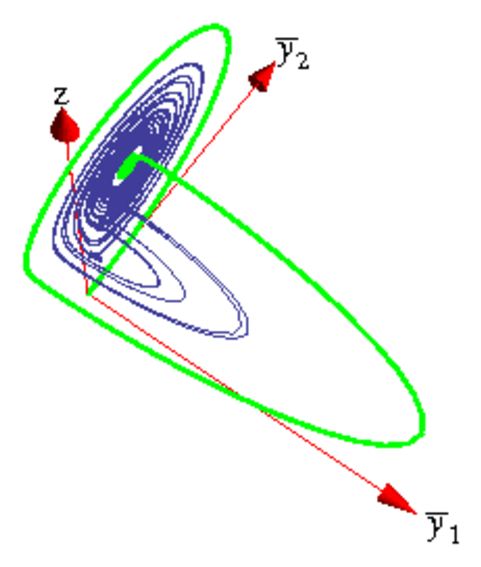
\includegraphics[width=0.35\textwidth]{../figs/CLEmfYYZ}
\end{center}
\caption[Orbit space projection of Complex Lorenz flow: Moving frame]{ \Statesp\
portraits of \CLe\ dynamics for $e=1/10$, $\ImrCLor=0$
in \reducedsp. Projecting on invariants given in \refeq{eq:invLaser}.
    }
\label{fig:CLEmf}
\end{figure}
%%%%%%%%%%%%%%%%%%%%%%%%%%%%%%%%%%%%%%%%%%%%%%%%%%%%%%%%%%%%%%%%

In this section we illustrate symmetry reduction through 
the use of invariants computed 
with the moving frame method in the example of \CLe. 
The action \refeq{eq:SO2act} of $\SOn{2}$ on \Rls{5},
is regular on $\Rls{5}\backslash\{x_1=x_2=y_1=y_2=0\}$.
Thus we can define
a {\csection} by, for instance, 
\[
x_1=0,\,x_2>0\,. 
\]
We can now construct a moving frame for the action
\refeq{eq:SO2act} of $\SOn{2}$ as follows. We write out
explicitly the group transformations:
\begin{subequations}
\begin{align}
 	\overline{x}_1 &= x_1 \cos\theta - x_2 \sin\theta\label{eq:CLEexplSO2a}\cont
	\overline{x}_2 &= x_1 \sin\theta + x_2 \cos\theta\label{eq:CLEexplSO2b}\cont
	\overline{y}_1 &= y_1 \cos\theta - y_2 \sin\theta\label{eq:CLEexplSO2c}\cont
	\overline{y}_2 &= y_1 \sin\theta + y_2 \cos\theta\label{eq:CLEexplSO2d}\cont	
	\overline{z} &= z\,.
\end{align}
\end{subequations}
Then set $\overline{x}_1=0$ and solve
\refeq{eq:CLEexplSO2a} for the group parameter to obtain the moving frame
    \PC{is this text from around \refeq{eq:SO2stndMF} clipped in twice?}
\beq
	\theta=\tan^{-1}\frac{x_1}{x_2}
	\label{eq:CLEmf}
\eeq
which brings any point  back to the {\csection}.
Here it is important that
$\tan^{-1}$ distinguishes quadrants in the $(x_1,x_2)$ plane so the
transformation results to the correct geometric
interpretation.
Substituting \refeq{eq:CLEmf} in the remaining equations we
get the invariants
\beq
\begin{split}
	\overline{x}_2 &= \sqrt{x_1^2+x_2^2} = r_1 \cont
	\overline{y}_1 &= {(x_2 y_1-x_1 y_2)}/{r_1}\cont
	\overline{y}_2 &= {(x_1 y_1+x_2 y_2)}/{r_1}\,.
	\label{eq:invLaser}
\end{split}
\eeq
    \ES{The solution $\theta = 2
    \tan^{-1}\frac{-x_2+\sqrt{x_1^2+x_2^2}}{x_1}$ was
    returned by Mathematica. If we use $\theta =
    \tan^{-1}\frac{x_2}{x_1}$ without taking care of the
    quadrant our results are multiplied by $sgn(x_2)$.}
Note the relation to the invariant polynomials
\refeq{eq:ipLaser} and also that no syzygy is present.

On the other hand observe that the invariants are not well defined
in the limit of $x=x_1+i x_2$ approaching zero. 
Using $x=r_x\, e^{i\theta_x}\,,\, y=r_y\, e^{i\theta_y}$ we can write, 
for instance, $x_2 y_1-x_1 y_2 = r_x r_y \sin(\theta_x-\theta_y)$
and thus
\beq
        \overline{y}_1= r_y\sin(\theta_x-\theta_y)\,.
\eeq
Therefore, for any given $y$, the limit of $\overline{y}_1$ for $x \rightarrow 0$ 
does not exist, as the above expression depends on the direction
on the complex $x$-plane along which we approach zero. 
\ES{does not belong here: 
In terms of projecting dynamics 
on variables \refeq{eq:invLaser} (or applying the equivalent
procedure of rotating points back to the \slice) this means that
we need to take into account the direction along which
we approach zero and use the `angle
of descent' as the angle with which we rotate points back to the \slice, if such 
points have exactly $x=0$.
	} 
Note that the invariants are not defined on
the subspace $U_S$ defined by $x_1=x_2=0$ even though the
group action is non-regular only in a subset of $U_S$, the
$z$-axis $x_1=x_2=y_1=y_2=0$. The transformations
\refeq{eq:invLaser} can thus be characterized as
non-optimal, in the sense that we have singularity in a
proper superset of $\Fix{\SOn{2}}$. The reason the
transformations fail on $U_S$ and not only on the $z$-axis
can be traced back to the way we construct them. The action
of the group can be thought of as a direct sum of irreducible
actions and the corresponding invariant (irreducible)
subspaces are the $(x_1,\,x_2)$ and $(y_1,\,y_2)$
planes.
%PC OK \ES{Not sure if planes is acceptable term here.}.
The
fact the group acts on each irreducible subspace (that is, it
leaves it invariant as a set) implies that we could define a
moving frame in any one of them independently and the
singular subspace would only depend on the points on which
the action is not regular on this irreducible subspace. By
choosing an angle in the $(x_1,\,x_2)$ irreducible subspace
as the moving frame map, the singular set is the point
$x_1=x_2=0$ in this irreducible subspace, since the group
action is not regular, or alternatively, a polar
angle is not defined at that point. Going back to the full
$5$-dimensional space the singular set of the transformations
is still given by $x_1=x_2=0$.
%}

It is instructive to write \CLe~\refeq{eq:CLe} in the
variables \refeq{eq:invLaser}. This is achieved by using the
chain rule \refeq{ChainRul} and expressing the result in
terms of variables \refeq{eq:invLaser}. The equations now
read
\beq
\begin{split}
\dot{\overline{x}}_1 &= 0\,\\
\dot{\overline{x}}_2 &=-\sigma  \left(\overline{x}_2-\overline{y}_2 \right)\,,\\
\dot{\overline{y}}_1 &=-\overline{y}_1- \left(e+\sigma\frac{\overline{y}_1}{\overline{x}_2} \right)\overline{y}_2\,,\\
\dot{\overline{y}}_2 &=(\RerCLor -z)\overline{x}_2+\left(e+\frac{\sigma  \overline{y}_1}{\overline{x}_2}
\right) \overline{y}_1-\overline{y}_2\,,\\
\dot{z} &=\overline{x}_2 \overline{y}_2-b z\,.
\end{split}
\eeq
We again observe the singularity as
$\overline{x}_2\rightarrow 0$.
    \ES{We have done the same for ZM system long time ago when we
heuristically rederived Cartan's method. It has been moved to
a footnote in Jonathan's blog (eq. 5.37) and became one the
things that never found their way back to my thesis. One also
gets the same system by using invariant polynomials and
taking the syzygy into account, see discussion preceding 5.46
in Jonathan's blog. \\{\bf PC:} what was 'heuristic' about
it? It was an obvious idea that follows from interpretation
of dynamics in the fundamental domain for discrete
symmetries, we just did not know that it could be tracked
back at least to Poincar\'e. BTW, I never checked the
Poincar\'e reference, so I do not know whether the credit is
indeed due to him.
    }

The projections in \reffig{fig:CLEmf} reveal more about the
topology of the attractor but also present large ``jumps."
Note that the invariants \refeq{eq:invLaser} are related to
the invariant polynomials \refeq{eq:ipLaser} by division by
$\sqrt{x_1^2+x_2^2}$. This is the reason we get a clearer
visualization of the dynamics: All invariants scale
dimensionally as the original coordinates. At the same time
division by $\sqrt{x_1^2+x_2^2}$ causes the jumps in the
$\overline{y}$ components whenever the magnitude of $x$ comes
close to zero.

\PublicPrivate{}{
Geometrically we can interpret the jumps in the
$\overline{y}$ coordinates as follows: We have chosen to
measure angle on one of the irreducible subspaces of \SOn{2},
the $x$-plane, and project the dynamics on orbit space by
counter-rotating in both irreducible subspaces (the $x$- and
$y$-plane.) As long as a trajectory traces one lobe of the
Lorenz attractor the angle varies slowly and no problem
occurs. When a trajectory changes quadrant in the $x$-plane
to visit the almost opposite lobe (due to detuning we do not
visit the lobe related by rotation by $\pi$, in reality no
such thing exists) we get a rapid change in angle as the
trajectory passes close to the origin. In the $y$-plane we do
not necessarily change quadrant. Call $\Delta \theta_x$ and
$\Delta\theta_y$ the change in angle in the $x$- and
$y$-plane respectively, when the trajectory changes quadrant
in the $x$ plane. We always reduce to \reducedsp\ by
correcting by $-\Delta\theta_x$ instead of correcting by the
smallest angle.
}%end \PublicPrivate.

% Since $x$ cannot vanish
% The problem is mostly aesthetical in the present case,
% but for \KS\ system it will be important to prevent
% the denominator from vanishing.
%     \ES{Here I have a hunch that the denominator cannot
%     vanish but I can't prove it}
We observe that dynamics cannot enter $\Fix{\SOn{2}}$, \ie\
the $z$-axis, since {\fixedsp s} are flow invariant. Since
\SOn{2} representation in the \CLe\ example is a direct sum
of irreducible representations we cannot take more than one
irreducible subspace into account when setting up the
normalization equations, at least not in a convenient way. We
can however restore democracy between modes and extend
validity of the transformations to any point where the group
acts freely, by modifying the invariants as follows:
\beq
\begin{split}
	\overline{x}_2 &= (x_1^2+x_2^2)/r \cont
	\overline{y}_1 &= -(x_2 y_1-x_1 y_2)/r\cont
	\overline{y}_2 &=(x_1 y_1+x_2 y_2)/r\cont
	\overline{z} &=z\cont
	r &= \sqrt{x_1^2+x_2^2+y_1^2+y_2^2}
    \,.
	\label{eq:invLaser2}
\end{split}
\eeq
This set of invariants lacks a geometric interpretation\ES{or
does it?} but results in much cleaner phase portraits, \cf
\reffig{fig:CLEinv}.


%%%%%%%%%%%%%%%%%%%%%%%%%%%%%%%%%%%%%%%%%%%%%%%%%%%%%%%%%%%%%%%%%%
\begin{figure}[ht]
\begin{center}
  (\textit{a})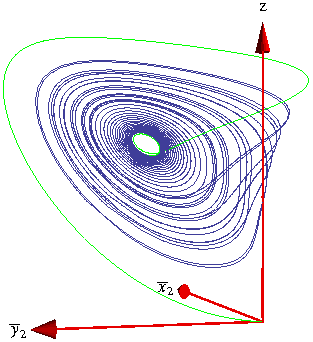
\includegraphics[width=0.35\textwidth]{../figs/CLEinvXYZ}
~~~~(\textit{b})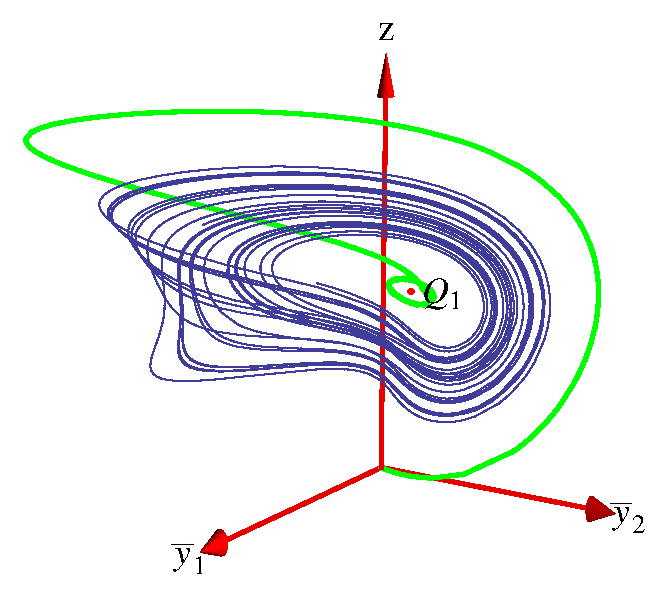
\includegraphics[width=0.35\textwidth]{../figs/CLEinvYYZ}
\end{center}
\caption{
\Statesp\ portraits of \CLe\ dynamics for $e=1/10$,
$\ImrCLor=0$ in \reducedsp. Projecting on invariants given in
\refeq{eq:invLaser2}.
    }
\label{fig:CLEinv}
\end{figure}
%%%%%%%%%%%%%%%%%%%%%%%%%%%%%%%%%%%%%%%%%%%%%%%%%%%%%%%%%%%%%%%%

%%%%%%%%%%%%%%%%%%%%%%%%%%%%%%%%%%%%%%%%%%%%%%%%%%%%%%%%%%%%%%%%%%
\begin{figure}[ht]
\begin{center}
%   (\textit{a})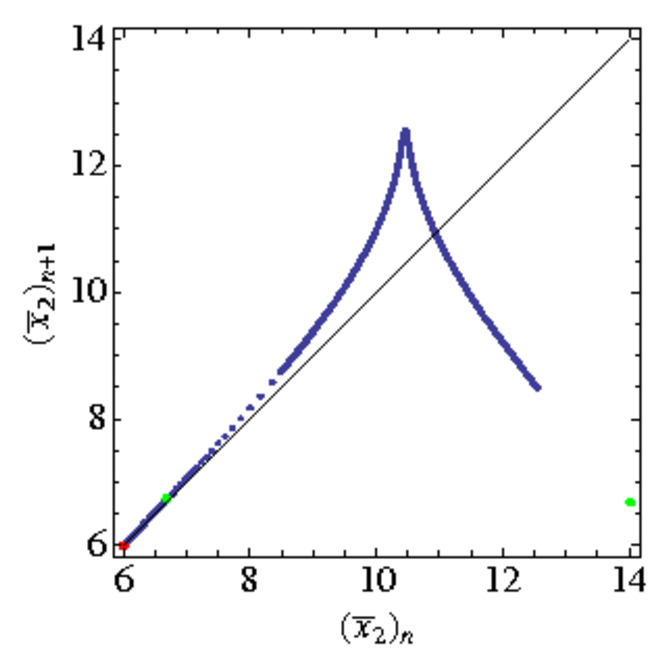
\includegraphics[width=0.35\textwidth]{../figs/CLEinvRMx2}
%  ~~~~(\textit{b})
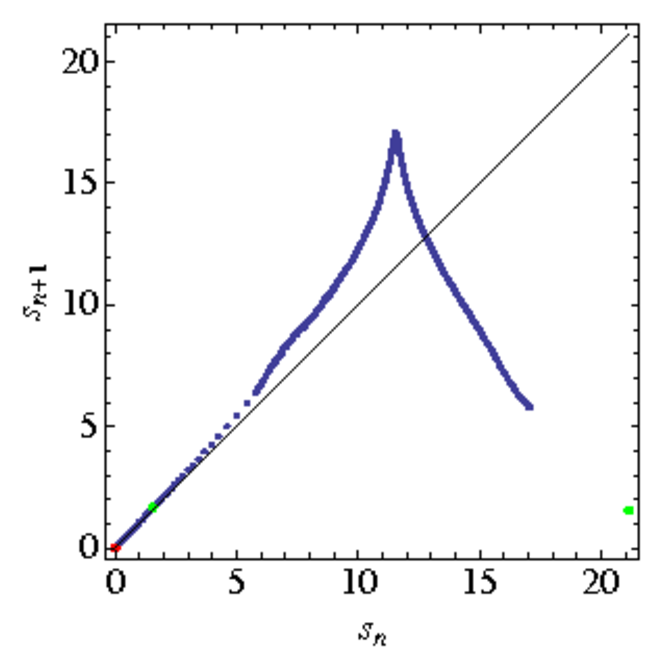
\includegraphics[width=0.35\textwidth]{../figs/CLEinvRM}
\end{center}
\caption[Return map for Complex Lorenz flow]{
Return map to the \Poincare\ surface of section
$\overline{x}_2=\overline{y}_2$ for \CLe\ with $e=1/10$,
$\ImrCLor=0$, projecting on invariants given in
\refeq{eq:invLaser2}. The return map coordinate is the
Euclidean length along the \Poincare\ section of the unstable
manifold of $E_1$.
    }
\label{fig:CLEinvRM}
\end{figure}
%%%%%%%%%%%%%%%%%%%%%%%%%%%%%%%%%%%%%%%%%%%%%%%%%%%%%%%%%%%%%%%%
